\section{Client-Server Interaction}
When a lecturer creates a new exercise, a modal prompts to enter details about the exercise.
These details include the name of the exercise, instructions for the student, an optional code template to help the student get started, as well as test code.
This data is sent to the database where it is stored.
When a student opens an exercise, the data is then fetched from the database.
This is done by the client sending a request to the Next.js backend, which queries the database and returns both exercise and test data.

\begin{figure}[H]
    \centering
    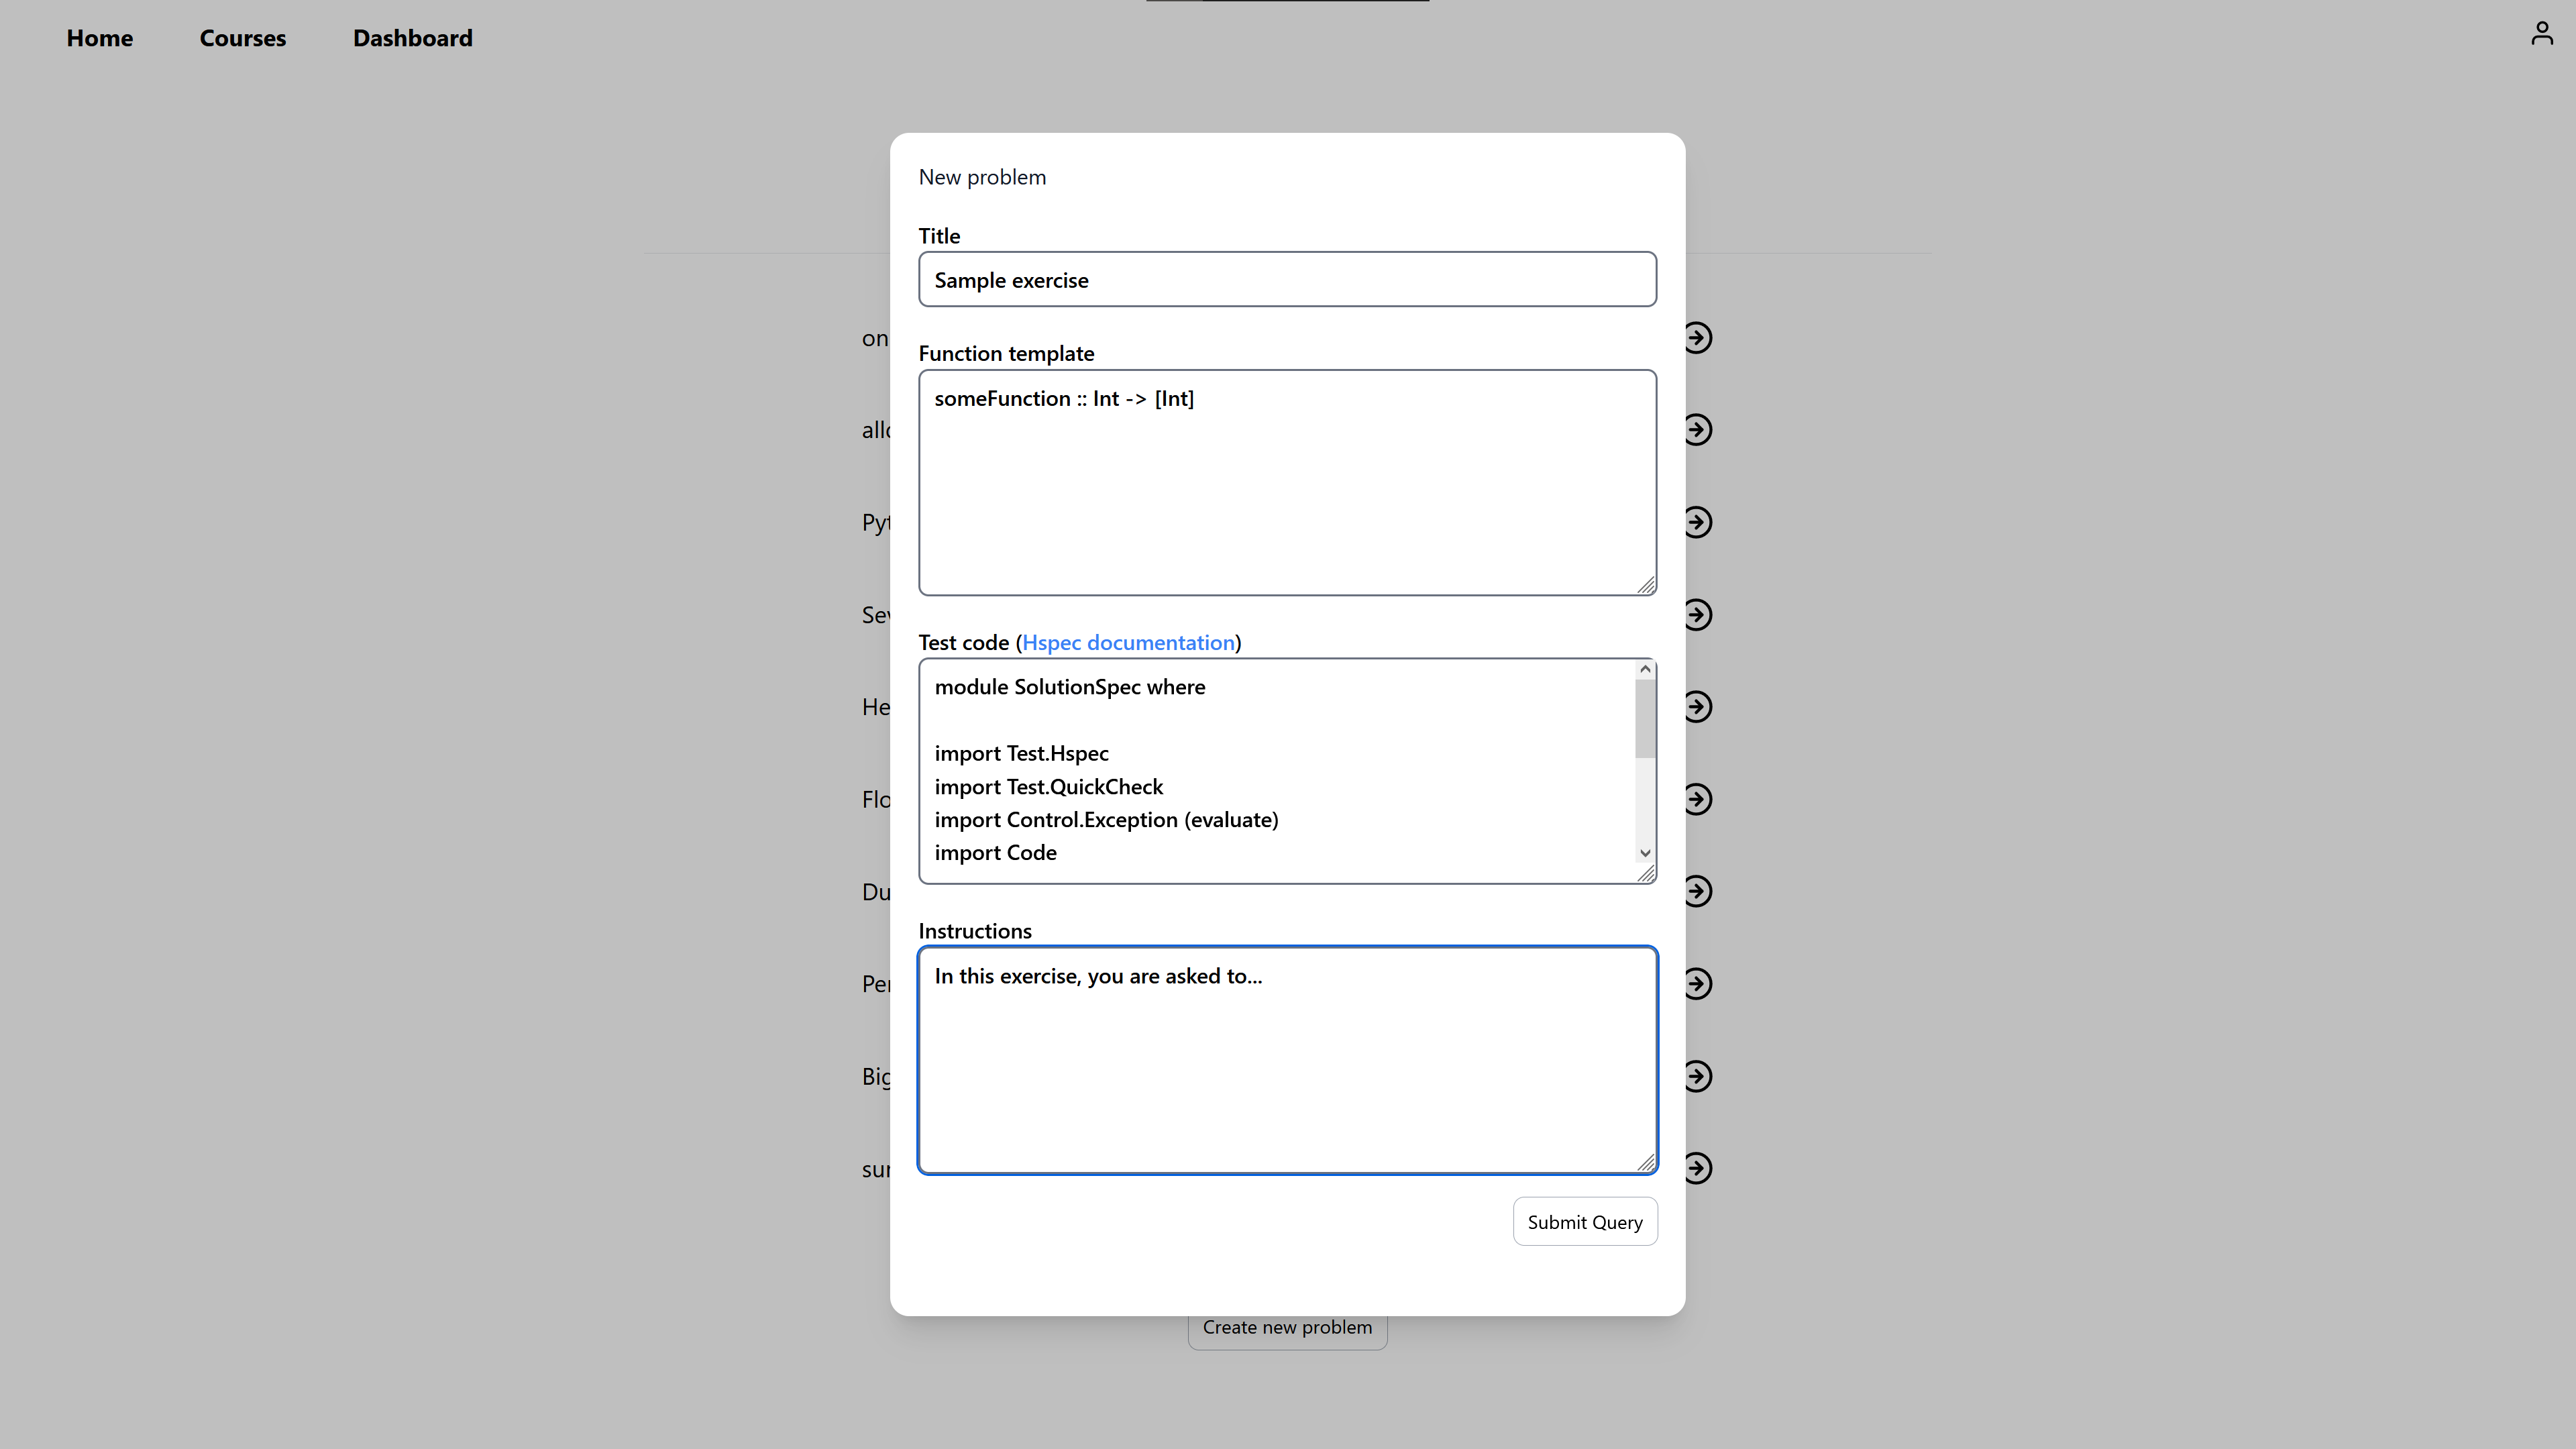
\includegraphics[scale=0.1]{create_exercise.png}
    \caption{Creating a new exercise as a lecturer}
    \label{fig:create_exercise}
\end{figure}

In the interest of reducing the number of database queries, the result of this request is cached on the client.
The client will eagerly request new data to stay up to date with instructions or test code updates.
This short cache storage time is useful for when lecturers update test code during an exercise session.
This way, all students have the latest test code shortly after the update while still minimizing unnecessary queries.

When a user submits their exercise solution attempt, a mutation is sent to the Next.js backend.
In this request, the code and test is included.

To handle this mutation, the Next.js server requests the Test Runner to process the given solution and test code.
This process is described in chapter \ref{chap:TestRunner}.
The response of this request to the Test Runner is validated and stored as a submission in the database.
This allows users and lecturers to access previous submissions, which includes code and a value indicating whether the submission satisfied the exercise tests.
Lastly, the result is sent to the client and displayed on the page.
if the submission solves the problem a success message is displayed, otherwise an error message is shown, this can be seen on figure \ref{fig:exercise_success} and \ref{fig:exercise_fail} respectively.
Images of the platform's user interface can be seen in appendix \ref{chap:images}.

\begin{figure}[H]
	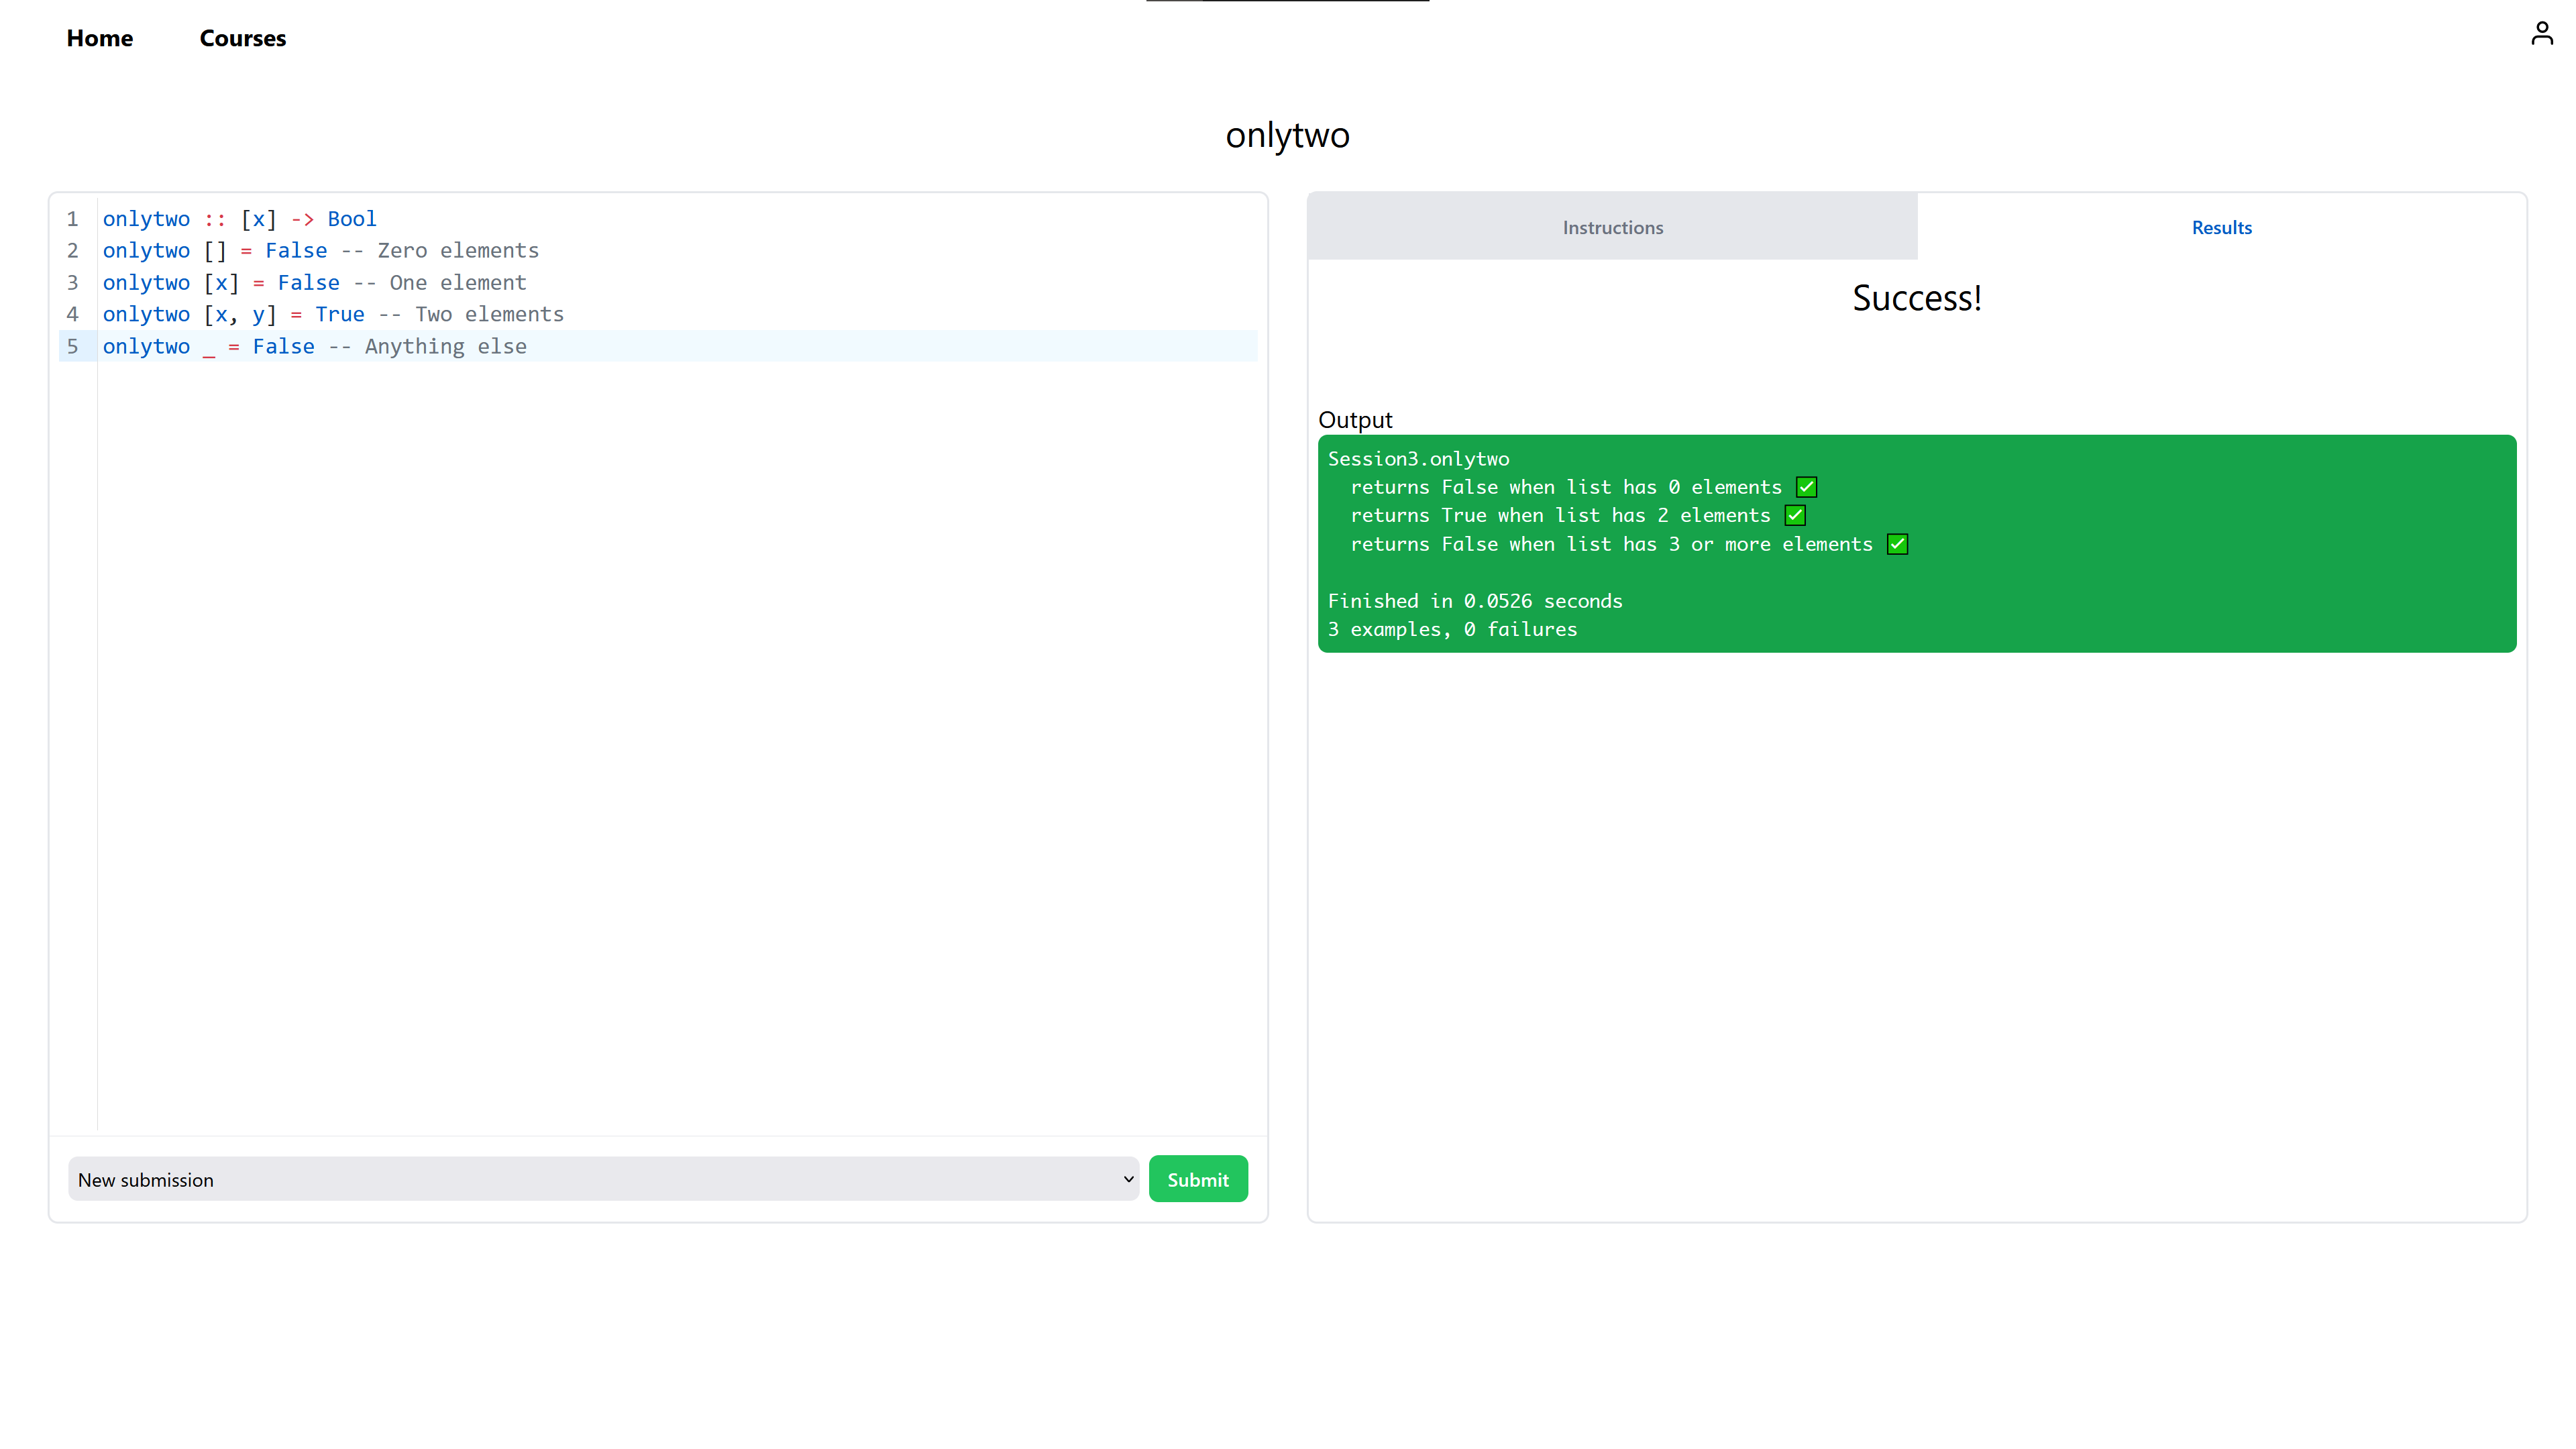
\includegraphics[scale=0.1]{exercise_success.png}
	\centering
	\caption{An example of a successful exercise submission}
	\label{fig:exercise_success}
\end{figure}

\begin{figure}[H]
	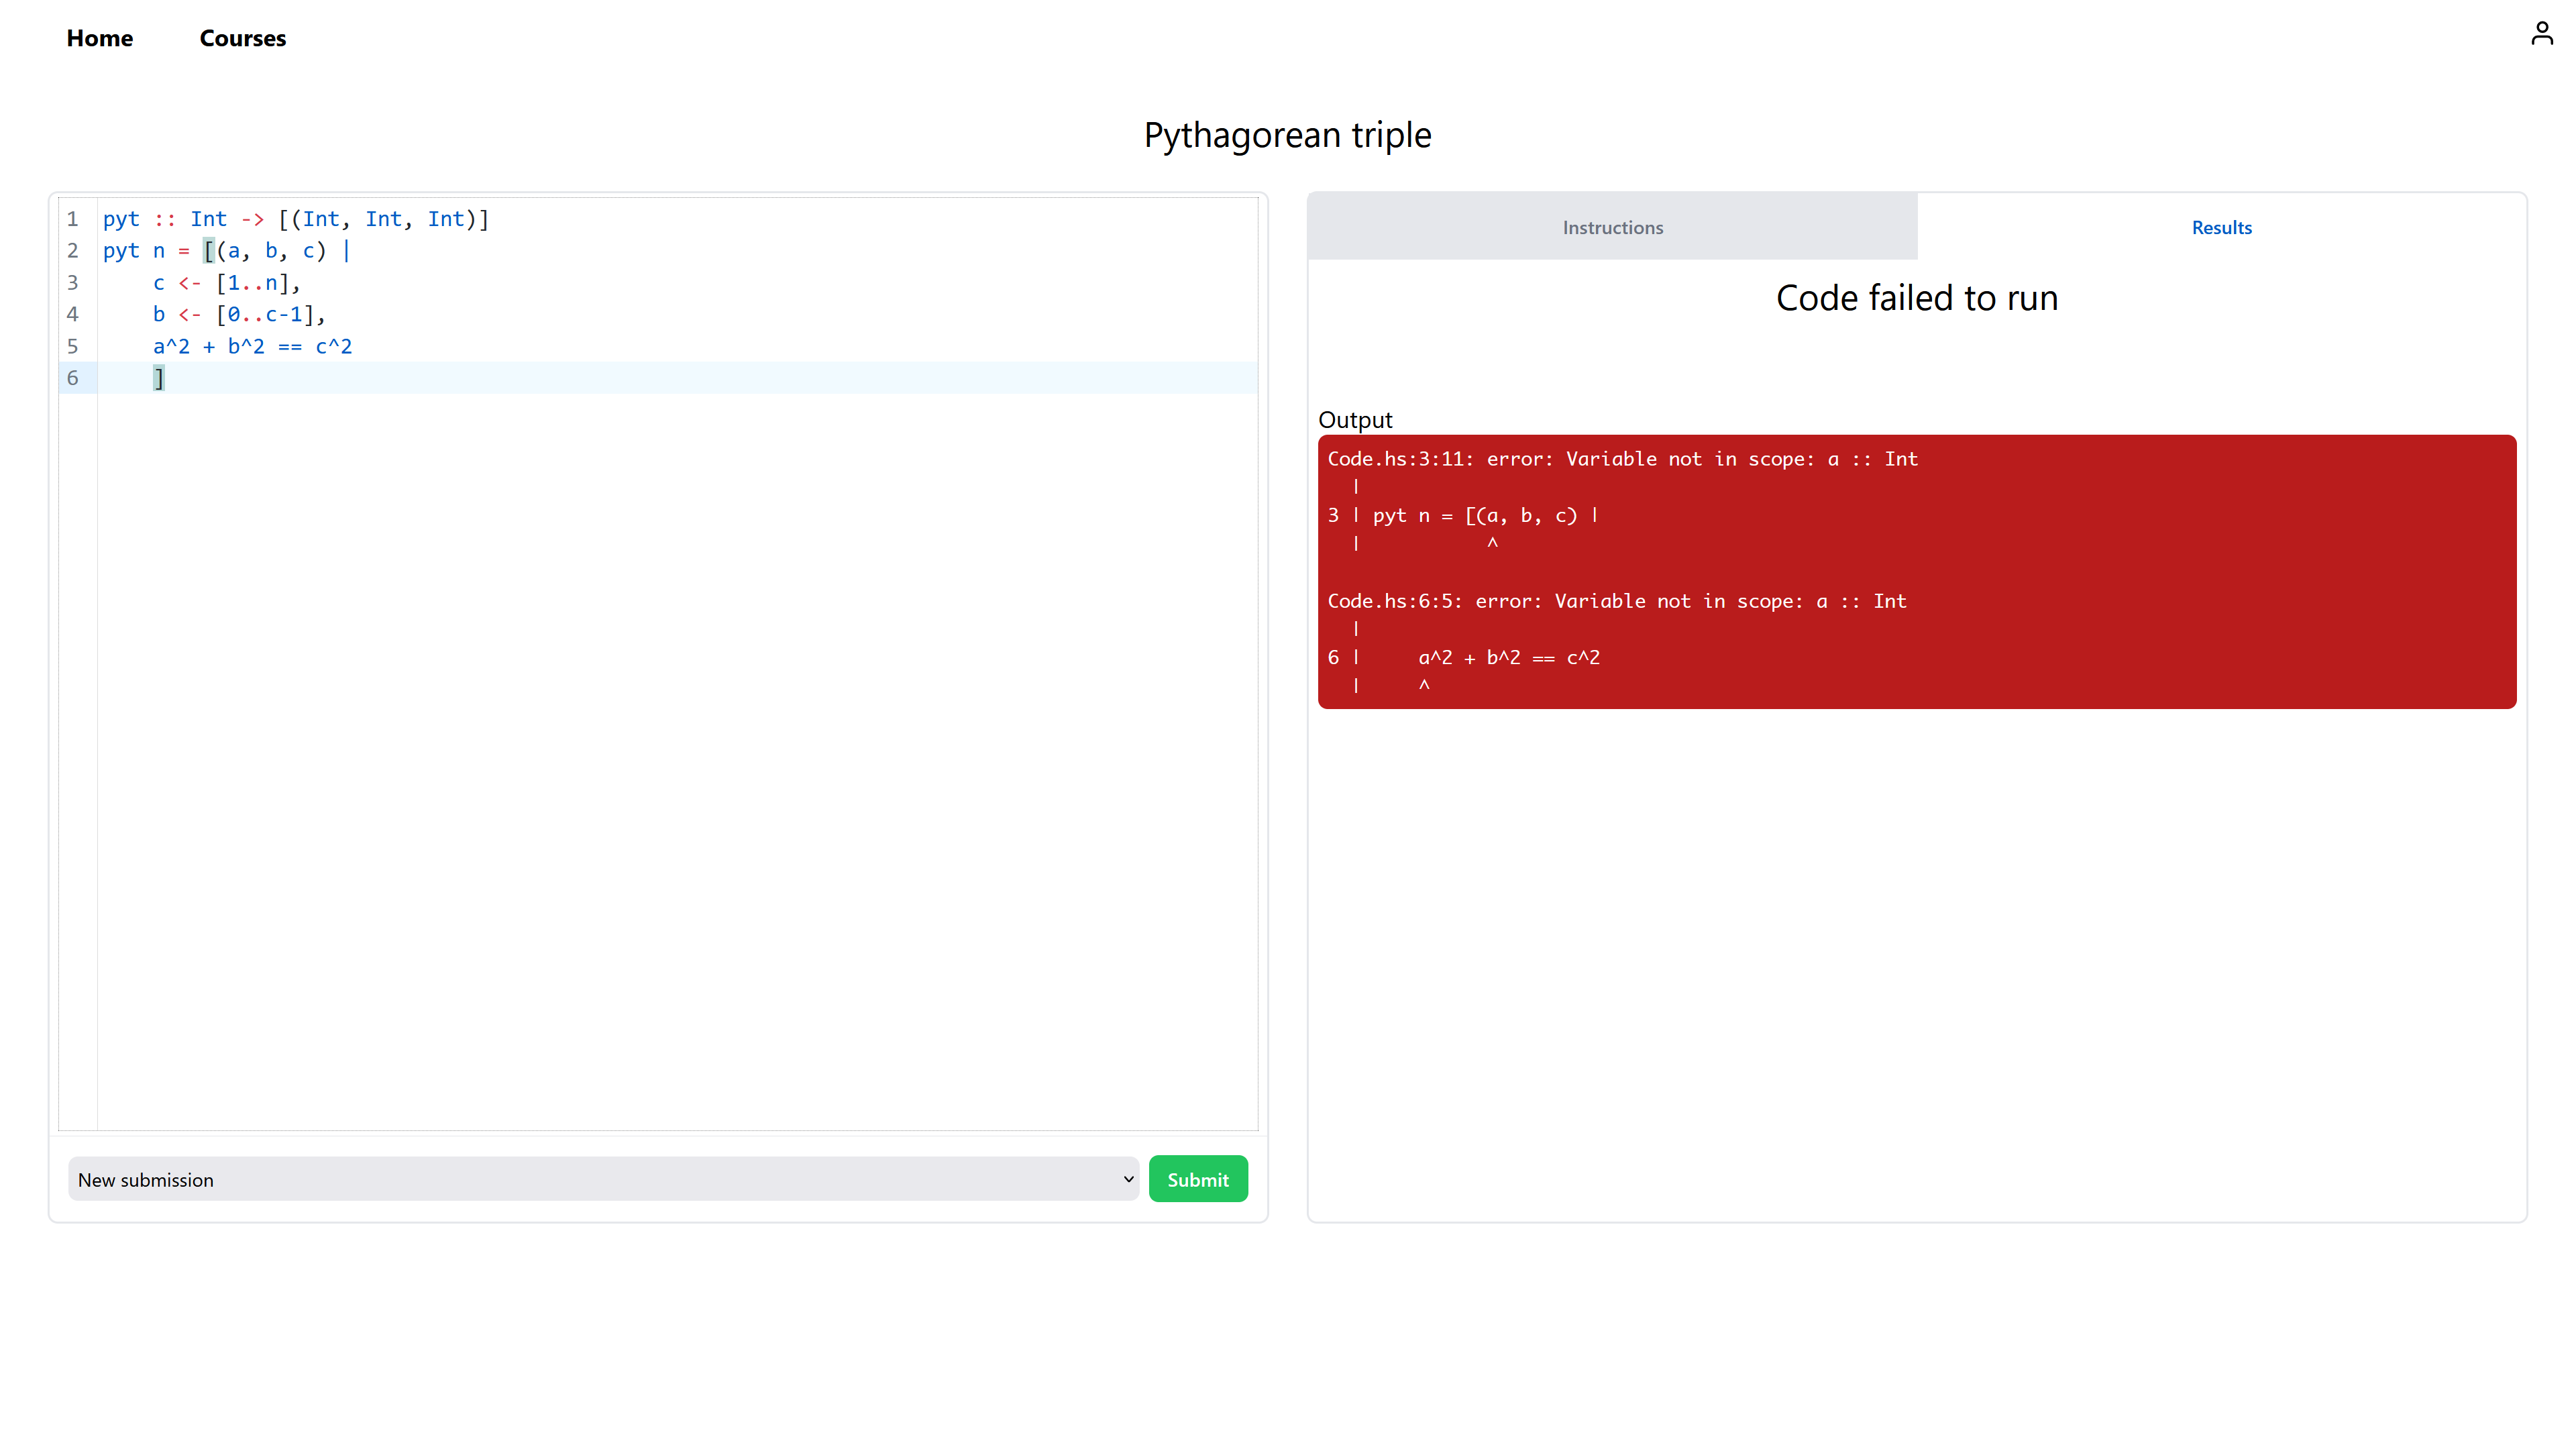
\includegraphics[scale=0.1]{exercise_fail.png}
	\centering
	\caption{An example of an unsuccessful exercise submission}
	\label{fig:exercise_fail}
\end{figure}
